% DO NOT COMPILE THIS FILE DIRECTLY!
% This is included by the other .tex files.

\section*{Outline}
\frame{\tableofcontents}

\section{Introduction}

\begin{frame}[t]{}
\vskip80pt
\begin{center}
\Huge Computational Humor  
\end{center}
\end{frame}

\begin{frame}[t]{}
\vskip80pt
\begin{columns}[c]
  \column{1.9in}
  \centering
    \only<2> {$ \underbrace{\text{\Huge Computational}}_{}$ \vskip34pt $\sim$ The possibility of being modeled on a computer.}
  \column{1.5in}
  \centering
  $ \underbrace{\text{\Huge Humor}}_{}$ \vskip2pt The tendency of particular cognitive experiences to provoke laughter and provide amusement.
\end{columns}

\note{
In science, cognition is a group of mental processes that includes attention, memory, producing and understanding language, learning, reasoning, problem solving, and decision making.
Cognition is a faculty for the processing of information, applying knowledge, and changing preferences. 
Cognition, or cognitive processes, can be natural or artificial, conscious or unconscious. 
}

\end{frame}



\begin{frame}[t]{Why computational humor?}
% Humor affects attention and memory, facilitates social interaction,
% and ameliorates communication problems. If computers are ever
% going to communicate naturally and effectively with humans, they
% must be able to use humor. Moreover, humor provides insight into
% how humans process language—real, complex, creative language,
% not just a tractable subset of standard sentences. By modeling humor
% generation and understanding on computers, we can gain a better
% picture of how the human brain handles not just humor but language
% and cognition in general.

\begin{large}
\begin{itemize} 
  \item On the human side humor:
  \begin{itemize}
    \item Affects attention and memory. 
    \item Facilitates social interactions.
  \end{itemize}
  \item Under a research point of view, humor modeling:
  \begin{itemize}
    \item Is an \emph{AI-complete} problem.
    \item Could give insights into how humans process real, complex, creative language.
  \end{itemize} 
\end{itemize}
\end{large}

\note{\begin{itemize}
        \item (Cognitive) Humor also has a positive effect on the mental state of
those using it and has the ability to improve their activity.
        \item (Computational) A successfully humorous computational system must:
          \begin{itemize}
            \item Recognize situa­tions appropriate for humor
            \item Choose a suitable kind of humor for the situation
            \item Generate humorous output
            \item Evaluate the feedback (if any)
          \end{itemize}
        \item (Computational) AI-Complete: As difficult as any other AI problem.
        \end{itemize}
}
\vskip80pt
\small \textbf{Source:}  \cite{binsted2006computational},\cite{stock2003getting}
\end{frame}

\begin{frame}[t]{Which are the fields concerned?}
  \begin{center}
    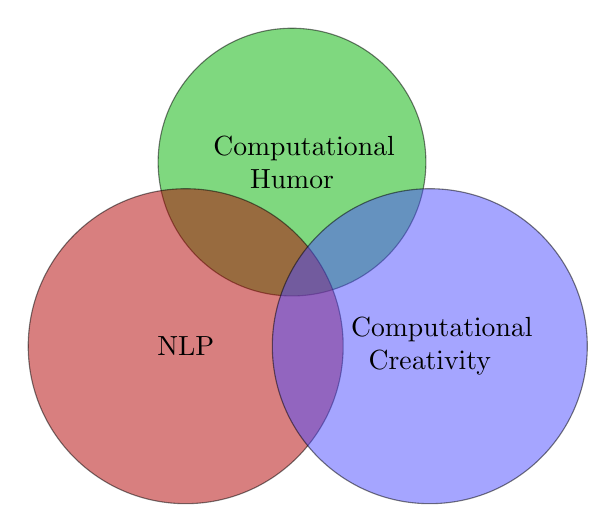
\begin{tikzpicture}
    \draw [fill=green!70!black,opacity=0.5] (60:2.7cm) circle (1.7cm) node [opacity=1,text width=2cm,align=center] {Computational Humor};
    \draw [fill=red!70!black,opacity=0.5] (0,0) circle (2cm) node [opacity=1] {NLP};
    \draw [fill=blue!70!white,opacity=0.5] (0:3.1cm) circle (2cm) node [opacity=1,text width=2cm,align=center] {Computational Creativity};
  \end{tikzpicture}  
  \end{center}
  
  \note{Subjects of interest \cite{}:
  \begin{itemize}
  \item Modeling verbal and nonverbal humor
  \item Recognizing and generating humor
  \item Embodied agents, social robots and humor
  \item Appropriateness of humor generation
  \item Nonverbal speech, facial expressions, and humor recognition
  \item Sentiment analysis and humor
  \item Humor corpora
  \item Applications of humor research
  \end{itemize} 
}
\end{frame}


\begin{frame}[t]{Which are the fields concerned?}
  \begin{center}
    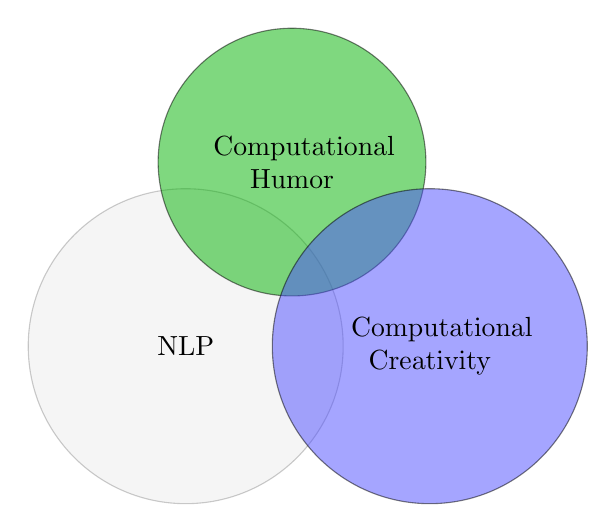
\begin{tikzpicture}
    \draw [fill=black!20,opacity=0.2] (0,0) circle (2cm) node [opacity=1] {NLP};
    \draw [fill=green!70!black,opacity=0.5] (60:2.7cm) circle (1.7cm) node [opacity=1,text width=2cm,align=center] {Computational Humor};    
    \draw [fill=blue!70!white,opacity=0.5] (0:3.1cm) circle (2cm) node [opacity=1,text width=2cm,align=center] {Computational Creativity};
  \end{tikzpicture}  
  \end{center}
  
  \note{}
\end{frame}


\section{Computational Creativity}

\begin{frame}[t]{What is computational creativity?}

\vskip50pt

\Large{Computational creativity is the \textbf<2>{study} and \textbf<2>{simulation}, by \textbf<2>{computational} means, of the behaviour, natural and artificial, which would, if observed in humans, be \textbf<3>{deemed creative}.} 
\begin{flushright}
\normalsize from \textit{The Association of Computational Creativity}
\end{flushright}

\note{The goal of computational creativity is to model, simulate or replicate creativity using a computer, to achieve one of several ends:
\begin{itemize}
  \item To construct a program or computer capable of human-level creativity
  \item To better understand human creativity and to formulate an algorithmic perspective on creative behavior in humans
  \item To design programs that can enhance human creativity without necessarily being creative themselves
\end{itemize}
}  
  
\end{frame}

\begin{frame}[t]{How is creativity defined?}
\begin{definition}
\begin{quotation}
\Large{"Creativity can be defined as the ability to generate \textbf<2>{novel} and \textbf<3>{valuable} ideas."}
\end{quotation}
\end{definition}
\vskip20pt
\only<2>{\large{
\textbf{Novelty}
\begin{itemize}
  \item Psychological - P-Creativity
  \item Historical - H-Creativity
\end{itemize}
\vskip60pt
\small \textbf{Source:}  \cite{boden2009computer},\cite{boden1998creativity}
}}
\only<3>{
\large{\textbf{Valuation}
\begin{itemize}
  \item Difficult to model
  \item Based on cultural and socially accepted style of thoughts.
  \item Subjective and dependant on motivation and emotional factors
\end{itemize}
\vskip40pt
\small \textbf{Source:}  \cite{boden2009computer},\cite{boden1998creativity}
}}
\vskip90pt
\onslide<1>{\small \textbf{Source:}  \cite{boden2009computer},\cite{boden1998creativity}}

  \note<2>{\begin{itemize}
    \item Mainly two types of creativity:
  \begin{itemize}
    \item \textbf{P-Creativity:} (Psychological or Personal) Novelty with respect to who made the invention.
    \item \textbf{H-Creativity:} (Historical) P-creative and never occurred in history before. 
  \end{itemize}
  \item Computer models aim at P-Creativity
  \end{itemize}}
  \note<3>{
  \begin{itemize}
  \item Valuable, here, has many meanings: interesting, useful, beautiful, simple, richly complex, and so on.
  \item Ideas is an umbrella term for (concepts,theories, interpretations, stories), but also artifacts such as graphic images, sculptures, houses, and jet engines).
  \item The structures generated within newly transformed spaces will need types of evaluation different (at least in part) from those implicit within the original space, or previously provided in explicit form.

  \end{itemize}
  }
\end{frame}

\begin{frame}[t]{How can creativity be achieved?}
\begin{itemize}
\onslide<2->{\item By \textbf{combination}
\begin{itemize}
\item Direct association of concepts that were previously unlinked ($\approx$ analogy)
\end{itemize}}
\onslide<3->{\item By \textbf{exploration}
\begin{itemize}
\item of a conceptual space (style of thinking)
\item defined by a set of generative rules
\end{itemize}}
\onslide<4->{\item By \textbf{transformation}
\begin{itemize}
\item of the conceptual space
\item by altering or dropping one of more of its defining dimensions (rules)
\end{itemize}}
\end{itemize}
\vskip20pt
\onslide<5->{A formal framework for the analysis of creative systems have been presented in \cite{wiggins2006preliminary}.}
\vskip25pt
\onslide<2->{\small \textbf{Source:} \cite{boden2009computer},\cite{boden1998creativity}}

\note<2-5>{\begin{itemize}
\only<3>{\item \textbf{Combination}
    \begin{itemize}
      \item Generally the most studied problem.
      \item Given a set of concepts, it is easy for a computer to combine them, but it is difficult to obtain valuable combination.
      \item AI Models of analogy: Domain-general mapping rules, applied to prestructured co concepts, generally based on a preexisting inter-linked knowledge base (or semantic networks) 
    \end{itemize}}
     
\only<4>{\item \textbf{Exploration}
    \begin{itemize}
      \item Exploration rules must be computable.
      \item Exploration rules are determined by AI skills along with expertise in the domain.
      \item Exploration assume the existence of a general theoretical framework. 
    \end{itemize}}

\only<5>{\item \textbf{Transformation}
    \begin{itemize}
      \item $\sim$ Exploration at a meta-level.
      \item May involve self-modification of the creative agent.
      \item Generally difficult to automate.
    \end{itemize}}
    
\only<5>{\item All the definitions tries to map the creative process to some interaction with a search space.
    \item Two major bottlenecks:
    \begin{itemize}
      \item \textbf{Domain-expertise:} Required for mapping the conceptual space that is to be explored and/or transformed.
      \item \textbf{Results valuation:} Necessary and especially difficult for transformational programs.
    \end{itemize}}
    
  \end{itemize}}
\end{frame}

\begin{frame}[t]{Successful examples}
  \begin{itemize}
  \item \textbf{Combinational creativity}
  \begin{itemize}
  \item JAPE : A program for producing punning riddles \cite{binsted1996machine} 
  \end{itemize}
  \item \textbf{Exploratory creativity}
  \begin{itemize}
  \item EMI : Experiments in musical intelligence \cite{cope1991computers}
  \item Jazz improvisation in the style of Charlie Parker \cite{hodgson2005modelling}
  \item AARON : Line drawing and coloring painter \cite{cohen1995further}
  \item BACON : Heuristic-based suite to model scientific discovery \cite{stacey1988scientific}
  \end{itemize}
  \item \textbf{Transformational creativity}
  \begin{itemize}
  \item Automated Mathematician \cite{lenat1983role}
  \item Eurisko \cite{lenat1983role}
  \end{itemize}
  \end{itemize}
  
  \note{\begin{itemize}
  \item \textbf{Combinational creativity}
  \begin{itemize}
  \item \begin{scriptsize}
  Joke forms: What do you get when you cross X with Y?;  What’s the difference between an X and a Y? The semantic network used by the program incorporates knowledge of phonology,semantics, syntax, and spelling. 
  \end{scriptsize}
  \end{itemize}
  \item \textbf{Exploratory creativity}
  \begin{itemize}
  \item \begin{scriptsize}
  EMI : Program that composes in the styles of Mozart, Stravinsky, Joplin, and others.In order to do this, it employs powerful musical grammars expressed as ATNs.
  \end{scriptsize}
  \item {\scriptsize Besides strong (and relatively general) knowledge of musical dimensions such as harmony and rhythm, and of musical conventions characteristic of jazz, the system has access to a large set of Parker-specific motifs, which can be varied and combined in a number of ways.} 
  \item \begin{scriptsize}
  AARON cannot reflect on its own productions,nor adjust them so as to make them better.
It cannot even transform its conceptual space. 
In this, it resembles most current AI-programs focused on creativity.
  \end{scriptsize}
 
  \end{itemize}
  \item \textbf{Transformational creativity}
  \begin{itemize}
  \item {\tiny Both consists of heuristics, i.e. rules of thumb, including heuristics describing how to use and change its own heuristics.}
  \end{itemize}
  \end{itemize}}
\end{frame}

\section{Computational Humor}

\begin{frame}[t]{Why CH is AI-Complete?}
\begin{large}
A successfully humorous computational system should be able to:
\begin{enumerate}
  \item Recognize situa­tions appropriate for humor.
  \item Choose a suitable kind of humor for the situation.
  \item Generate an appropriately humorous output.
  \item (In case of interaction or control) Evaluate the feedback.  
\end{enumerate}
\end{large}
\vskip75pt
\small \textbf{Source:}  \cite{stock2003getting}
  \note{ Relations between computational creativity and computational humour:
\begin{itemize}
  \item Automatic discovery of humor.
  \item Automatic creation of humor expressions.
  \item Semiautomatic collaborative human-computer creation of humor.
  \item Automatic appreciation and evaluation of humor production.
\end{itemize}
}
\end{frame}

\begin{frame}[t]{Which AI fields are concerned?}
\vskip15pt
\begin{Large}
\begin{itemize}
  \item \textbf{Humor generation} \onslide<2->{$\longmapsto$ \textbf{Computer Creativity}}
  \begin{itemize}
    \item Choose a suitable kind of humor for the situation.
    \item Generate an appropriately humorous output. 
  \end{itemize}
\end{itemize}
\vskip20pt
\begin{itemize}
  \item \textbf{Humor detection} \onslide<3->{$\longmapsto$ \textbf{NLP}}
  \begin{itemize}
    \item Recognize situa­tions appropriate for humor.
    \item (In case of interaction or control) Evaluate the feedback. 
  \end{itemize}  
\end{itemize}

\end{Large}
  \note{}
\end{frame}

\begin{frame}[t]{CH State-of-the-art}

{\Large\textbf{Current research}}
\vskip20pt
\begin{Large}
\begin{itemize}
  \item \textbf{Humor Production}
  \begin{itemize}
    \item \href{http://haha.fbk.eu/}{Humourous Agent for Humorous ACRONYMNs} - European Project IST-2000-30039.
    \item  Computational Humour for Creative Naming
  \end{itemize}
  \vskip10pt
  \item \textbf{Humor Recognition and Understanding}
   \begin{itemize}
    \item Corpus-based methods for humor recognition  
  \end{itemize}
  \vskip10pt
  \item \textbf{Humour in User Interfaces}
\end{itemize}
\end{Large}
\vskip40pt
\small \textbf{Source:}  \cite{mulder2002humour} \cite{nijholt2012computational}

\note{
\begin{scriptsize}
\begin{itemize}  
  \item \textbf{Humor Production}
  \begin{itemize}
    \item \href{http://haha.fbk.eu/}{Humourous Agent for Humorous ACRONYMNs} - European Project IST-2000-30039.
    \item  Computational Humour for Creative Naming
  \end{itemize}
  \item \textbf{Humor Recognition and Understanding}
   \begin{enumerate}
    \item Collect a sufficiently large set of humorous text (corpus).
    \item Apply classification methods (mainly supervised) across different data sets.
    \item Analyze the results to determine whether some humor distinctive features exists or not.
    \end{enumerate}
  \item \textbf{Humour in User Interfaces}
  \begin{itemize}
    \item The study provides strong evidence that humour should be incorporated in CMC and HCI systems, since the user responded to the system in a more sociable manner and reported greater cooperation.
  \end{itemize}
\end{itemize}
\end{scriptsize}}
     

\end{frame}

\begin{frame}[t]{CH Research}

{\Large\textbf{Future research}}
\vskip20pt
\begin{Large}
\begin{itemize}
  \item \textbf{Formal theory}
  \vskip10pt
  \item \textbf{Multimodality}
  \vskip10pt
  \item \textbf{Sociality and Evaluation}  
\end{itemize}
\end{Large}
\vskip70pt
\small \textbf{Source:}  \cite{mulder2002humour} \cite{nijholt2012computational}
 
 \note{\begin{scriptsize}
 \begin{itemize}
   \item \textbf{Theory:} Theories that describe the creative process, are needed, eventually relating novelty with revisitation of known material.
   \item \textbf{Humor Production:} Combining top down rule-based approaches, which model general strategies, and learning from corpora.
   \item \textbf{Multimodality and new forms of humor:} Novel kind of forms of humor may possibly be introduced with the potential provided by new devices that bring about novel forms of multimodal interaction.
   \item \textbf{Sociality:} A key element for humor success is deciding when the situation is appropriate for humorous interventions. Research on computational models to detect whether the context is favorable and the effects of humor are those expected.
 \end{itemize}
     
\end{scriptsize}
}
\end{frame}

\begin{frame}[t,fragile]{Applications}
\begin{large}
\begin{itemize}
  \item A few programs implementing  models of humor exists (cf. \cite{mulder2002humour} \cite{nijholt2012computational}).
  \vskip20pt
  \item Unfortunately, they are mostly proofs of concept.
  \vskip20pt
  \item Applications of computational humor can be foreseen in:
  \begin{itemize}
    \item Advertisement (targeted)
    \item Human-Computer Interaction
  \end{itemize}
\end{itemize}
\end{large}
\note{
\begin{itemize}
  \item STANDUP Interactive Riddle-Builder helps children with communication-related disabilities use humor to interact with other children.
  \item Joke Analysis and Production Engine. Elmo, the Natural Language Robot. The Light Bulb Joke Generator. The Mnemonic Sentence Generator. 
\end{itemize}}
\end{frame}


\begin{frame}[t,fragile]{Conclusions}
{\Large \textbf{Computational Humor:}}
\begin{itemize}
  \item Is a relatively new field of research ($<$ 15 years).
  \item Is based on humor research in psychology, philosophy, linguistics, sociology, history and literature as well as computational linguistics and artificial intelligence.
  \item May yield to a more emphatic and sociable HCI.
  \item Tries to understand (and thus model) the roots of creative language. 
\end{itemize}
\vskip20pt
\begin{center}
\textit{"A conclusion is simply the place where you got tired of thinking."} - Anonymous
\end{center}
\end{frame}
 
\begin{frame}[t,fragile]{Questions?}
\begin{center}

\includegraphics[height=.8\textheight,keepaspectratio]{UlbLogos/Questions.jpg}
\end{center}
\end{frame}


% \begin{frame}[t,fragile]{User-based segmentation}
% \begin{center}
% \includegraphics[height=.8\textheight,keepaspectratio]{AutomationSchema}
% \end{center}
% \end{frame}

% \begin{frame}[t,fragile]{Strategies overview}
% \begin{itemize}
% \item \textbf{Strategy 1 -} Deterministic choice of ground truth objects centers as seed points.
% \item \textbf{Strategy 2 -} Non-deterministic choice of seeds points with distance-proportional probability.
% \item \textbf{Strategy 3 -} Computation of the shortest seed line defining an acceptable segmentation.
% \item \textbf{Strategy 4 -} Computation of the shortest seed line defining an acceptable segmentation with preference for those passing near the center of the object.
% \end{itemize}
% \end{frame}

% \begin{frame}[t,fragile]{Automated Strategy 1 - Overview}
% Seed points are chosen in a way that :
% \begin{itemize}
%   \item \textbf{(Initialization) -}Intuitively, points closer to the center of the ground truth object are marked as object point, while points clearly outside of it are marked as background
%   \item \textbf{(Update) -} Update seed points are chosen within large misclassified areas
% \end{itemize}
% \textbf{Strong points :}
% \begin{itemize}
%   \item Efficient computation using fast 2D Euclidian distance. 
%   \item Determinism.
%   \item Useful baseline for comparisons.
% \end{itemize}
% \textbf{Weak points :}
% \begin{itemize}
%   \item Determinism does not allow to test the robustness of the strategy.
%   \item Seeds have the form of pixel blobs instead of curves.
% \end{itemize}
% \end{frame}


% \begin{frame}[t,fragile]{Automated Strategy 2 - Overview}
% The strategy is similar to the previous one, the main difference being a non deterministic choice of the points according to a probability distribution which is proportional
% to the distance of points within the candidate set to points outside this set. \newline
% \textbf{Strong points :}
% \begin{itemize}
%   \item Efficient computation using inversion method to compute the probability.
%   \item Non-Determinism allows to test repeatability, hence robustness.
% \end{itemize}
% \textbf{Weak points :}
% \begin{itemize}
%   \item Seeds have the form of pixel blobs instead of curves.
% \end{itemize}
% \end{frame}

% \begin{frame}[t,fragile]{Automated Strategy 1-2 - Example}
% \begin{center}
% \includegraphics[height=.8\textheight,keepaspectratio]{Strategy1Ex}
% \end{center}
% \end{frame}


% \begin{frame}[t,fragile]{Automated Strategy 3 - Overview}
% The seed set will have the form of an automatically generated line, obtained by applying Dijkstra's shortest path algorithm on the adjacency graph of the candidate pixels.
% The line will be eventually expanded using a brush function to ensure a better coverage of the object.\newline
% \textbf{Strong points :}
% \begin{itemize}
%   \item Efficient computation of connection relationship and shortest path using Dijkstra's algorithm.
%   \item Seed line define a better coverage of the ground truth object than pixel blobs.
% \end{itemize}
% \textbf{Weak points :}
% \begin{itemize}
%   \item Shortest seed line tends to be closer to the border than desired.
% \end{itemize}
% \end{frame}

% \begin{frame}[t,fragile]{Automated Strategy 3 - Example}
% \begin{center}
% \includegraphics[height=.5\textheight,keepaspectratio]{Strategy3Ex}
% \end{center}
% \end{frame}

% \begin{frame}[t,fragile]{Automated Strategy 4 - Overview}
% This strategy is identical to the previous one, except for the weight assigned to each edge in the adjacency graph, which is modified in order to produce
% seed lines which pass closer to the center of the ground truth object.\newline
% \textbf{Strong points :}
% \begin{itemize}
%   \item Efficient computation of connection relationship and shortest path using Dijkstra's algorithm.
%   \item Seed line define a better coverage of the ground truth object than pixel blobs.
% \end{itemize}
% \textbf{Weak points :}
% \begin{itemize}
%   \item Shortest seed line tends to be closer to the border than desired.
% \end{itemize}
% \end{frame}

% \begin{frame}[t,fragile]{Automated Strategy 3 - Example 1}
% \begin{center}
% \includegraphics[height=.5\textheight,keepaspectratio]{Strategy3Ex2}
% \end{center}
% \end{frame}

% \begin{frame}[t,fragile]{Automated Strategy 3 - Example 2}
% \begin{center}
% \includegraphics[height=.7\textheight,keepaspectratio]{Strategy4Ex}
% \end{center}
% \end{frame}

% \section{Results Analysis}
% \begin{frame}[t,fragile]{Evaluation method}
% Given an input image and the corresponding ground truth:
% \begin{enumerate}
% \item Select strategy and algorithm.
% \item Process image according to strategy and algorithm.
% \item Compute object accuracy and border accuracy.
% \item Update seeds.
% \item If maximum step number has been reached stop, else goto 2.
% \end{enumerate}
% \begin{itemize}
%   \item Non deterministic strategy are rerunned 5 times in order to evaluate repeatability.
%   \item The maximum number of steps is equal to 100, which is unrealistic compared to human interaction, to allow stabilization of the results and to observe the strategy behavior over a long run.
%   \item Object and border accuracy will result in a time series of values.
%   \item Accuracy =  $\frac{TruePositive}{TruePositive+FalsePositive+FalseNegative}$ (Jaccard Index)
% \end{itemize}
% \end{frame}

% \begin{frame}[t,fragile]{Evaluation metrics}
% \begin{itemize}
%   \item \textbf{(Profile) - Time-Accuracy Profile } Average accuracy profile across time.
%   \item \textbf{(Aggregate) - Final Accuracy } Accuracy achievable across a reasonable amount of time.
%   \item \textbf{(Aggregate) - Integrated Accuracy } Accuracy integrated over time series data expanded in order to be comparable 
% \end{itemize}
% \begin{itemize}
%   \item These metrics can be averaged across all the object in the dataset to assess overall system performance.
%   \item Integrated accuracy is computed as a discrete summation of the area below the expanded time series.
%   \item Useful because it can be easily normalized with respect to the unity rectangle and briefly express the trend of average accuracy.
%   \item  Must be computed also for user interaction where steps are not unit spaced (i.e resampling or trapezoid rule).
% \end{itemize}
% \end{frame}

% \begin{frame}[t,fragile]{User Interaction Results}
% \begin{center}
% \includegraphics[height=.8\textheight,keepaspectratio]{MeanAccuracyUser}
% \end{center}
% \end{frame}

% \begin{frame}[t,fragile]{Automation Results - Accuracy Profile}
% \begin{center}
% \includegraphics[height=.8\textheight,keepaspectratio]{MeanAccuracyAutomation}
% \end{center}
% \end{frame}

% \begin{frame}[t,fragile]{Automation Results - Final Accuracy}
% \begin{center}
% \includegraphics[height=.7\textheight,keepaspectratio]{MeanAccuracyFinal}
% \end{center}
% \end{frame}

% \begin{frame}[t,fragile]{Automation Results - Integrated Accuracy}
% \begin{center}
% \includegraphics[height=.7\textheight,keepaspectratio]{MeanAccuracyIntegrated}
% \end{center}
% \end{frame}

% \begin{frame}[t,fragile]{Correlation metrics}
% \begin{itemize}
%   \item \textbf{Pearson's product-moment coefficient} 
%   \item \textbf{Spearman's $\rho$ rank coefficient}
% \end{itemize}
% \begin{itemize}
%   \item User (time-based) and automated (step-based) data must be aligned to perform correlation analysis.
%   \item Step-accuracy correlation analysis is limited to 60 step, because of results stabilization and limited number of user interactions.
%   \item Aggregated measures are averaged across different users (for human interaction) or different runs (for non-deterministic strategies) before performing correlation analysis.
%   \item High correlation between user and automated accuracy profile will show that the proposed method is well-emulating human behavior. 
% \end{itemize}
% \end{frame}

% \begin{frame}[t,fragile]{Automation Results - Step-accuracy correlation}
% \begin{center}
% \includegraphics[height=.6\textheight,keepaspectratio]{StepwiseCorrelation}
% \end{center}
% \end{frame}

% \begin{frame}[t,fragile]{Automation Results - Aggregate values correlation}
% \begin{center}
% \includegraphics[height=.7\textheight,keepaspectratio]{AggregateCorrelation}
% \end{center}
% \end{frame}

% \begin{frame}[t,fragile]{Conclusions}
% \begin{itemize}
% \item All the strategies have lead to results which are similar to those obtained with user segmentation.
% \item Strategy 3 and 4 have shown to be the most effective strategies at approximating real user input (highest rank correlation), with strategy 4 time accuracy profile having the closer visual correspondence with respect to user experiments one. 
% \item User evaluation is still the most effective way to evaluate interactive segmentation.
% \item Automated evaluation could provide useful and informative results whenever user test cannot be performed (e.g. due to high time consumption).
% \end{itemize}
% \end{frame}
